\subsection*{Question 1}

\begin{center}
	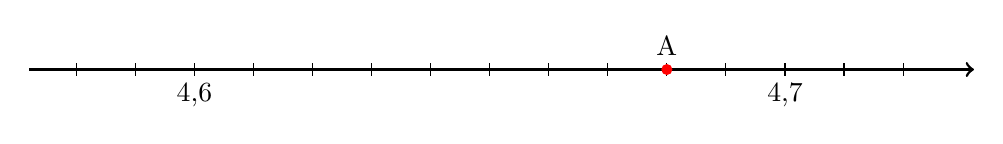
\begin{tikzpicture}[x=0.75cm]
		\draw[->,line width=1pt] (-2.8,0) -- (13.2,0);
		\foreach \i in {-2,...,12} \draw (\i,-0.08) -- (\i,0.08);
		\node[below] at (0,-0.05) {4,6};
		\node[below] at (10,-0.05) {4,7};
		\node[above] at (8,0.05) {A};
		\fill[red] (8,0) circle (2pt);
	\end{tikzpicture}
\end{center}

Entre 4,6 et 4,7, il y a un écart de 0,1 partagé en 10 graduations : une graduation vaut donc $0,1\div 10=0,01$.

Le point A est situé 8 graduations après 4,6 :
\[4,6+8\times 0,01=4,6+0,08=4,68.\]
L'abscisse du point A est 4,68.

\subsection*{Question 2 \quad Réponse C}

$4x+6x=10x$.

\subsection*{Question 3}

\og Ne pas obtenir une boule rouge \fg{} est l'évènement contraire de \og obtenir une boule rouge \fg{} :
\[P(\text{non rouge})=1-P(\text{rouge})=1-0,4=0,6.\]

\subsection*{Question 4}

7~h~10~min $+$ 53~min $=$ 7~h~63~min $=$ 8~h~03~min.

La voiture arrive à 8~h~03~min.

\subsection*{Question 5 \quad Réponse D}

Augmenter de 10\,\% revient à multiplier par $1+\dfrac{10}{100}=1,1$.
\[150\times 1,1=165.\]
Le nouveau prix est 165~\euro.

\subsection*{Question 6}

\begin{center}
	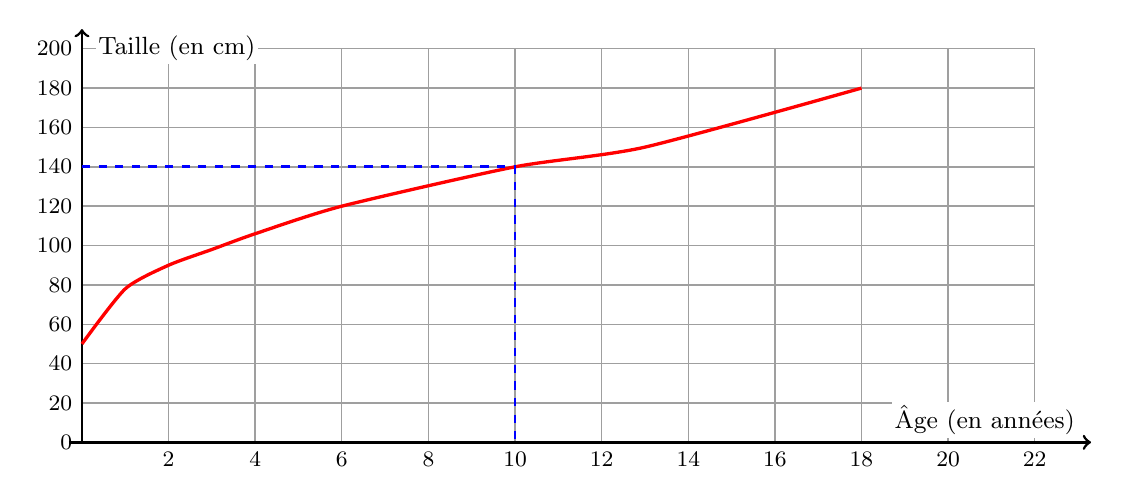
\begin{tikzpicture}[x=0.55cm,y=0.025cm]
		\draw[xstep=2,ystep=20,gray!75,line width=0.5pt] (0,0) grid (22,200);
		\draw[->,line width=1pt] (-0.3,0) -- (23.3,0);
		\draw[->,line width=1pt] (0,0) -- (0,210);
		\foreach \y in {0,20,...,200} \node[left] at (0,\y) {\footnotesize \np{\y}};
		\foreach \x in {2,4,...,22} \node[below] at (\x,0) {\footnotesize \np{\x}};
		\node[right,fill=white,inner sep=1pt] at (0.3,200) {\small Taille (en cm)};
		\node[above left,fill=white,inner sep=1pt] at (23,2) {\small Âge (en années)};
		\draw[red,line width=1.2pt] plot[smooth,tension=0.4] coordinates
		{(0,50) (1,78) (2,90) (3,98) (4,106) (6,120) (10,140) (13,150) (18,180)};
		\draw[blue,dashed,line width=1pt] (0,140) -- (10,140) -- (10,0);
	\end{tikzpicture}
\end{center}

La droite horizontale d'équation $y = 140$ coupe la courbe au point d'abscisse 10, et la courbe est au-dessus de cette droite après 10.

La taille de la personne a dépassé 140~cm à partir de 10 ans.

\subsection*{Question 7 \quad Réponse B}

Un nombre est divisible par 3 si la somme des nombres représentés par chacun de ses chiffres est divisible par 3 :

$9+5+4=18=3\times 6$, donc 954 est divisible par 3 ($954=3\times 318$).

\subsection*{Question 8 \quad Réponse A}

La somme des angles d'un triangle vaut $180^{\circ}$ :
\[\widehat{BAC}=180^{\circ}-47^{\circ}-53^{\circ}=80^{\circ}.\]

\subsection*{Question 9 \quad Réponse A}

Diviser par une fraction revient à multiplier par son inverse :
\[\dfrac{5}{8}\div\dfrac{8}{9}=\dfrac{5}{8}\times\dfrac{9}{8}=\dfrac{5\times 9}{8\times 8}=\dfrac{45}{64}.\]
